% !TEX program = xelatex
% DOFBOT 6軸アームの AIPL 実装 —— Capability 推論・TinyML・強化学習
\documentclass[11pt,a4paper]{article}

\usepackage[a4paper,margin=22mm]{geometry}
\usepackage{xeCJK}
\usepackage{fontspec}
\usepackage{amsmath,amssymb}
\usepackage{listings}
\usepackage{xcolor}
\usepackage{booktabs}
\usepackage{tabularx}
\usepackage{array}
\usepackage{graphicx}
\usepackage{hyperref}
\usepackage{enumitem}
\usepackage{pgfplots}
\pgfplotsset{compat=1.18}

\setCJKmainfont{Hiragino Mincho ProN}
\setCJKsansfont{Hiragino Sans}
\setCJKmonofont{Hiragino Sans}
\setmonofont{Menlo}[Scale=0.80]

% 丸数字(①..⑳)・水平線(―)・全角記号は CJK フォントで組む。
% 既定では欧文フォントに落ちて "Missing character" になり、字が消える。
\xeCJKDeclareCharClass{CJK}{"2015, "2190->"21FF, "2460->"24FF, "3000->"303F, "FF00->"FFEF}

\hypersetup{colorlinks=true, linkcolor=black, urlcolor=blue!60!black, citecolor=black}

\definecolor{kw}{RGB}{20,90,170}
\definecolor{cm}{RGB}{110,120,130}
\definecolor{st}{RGB}{20,120,60}
\definecolor{pr}{RGB}{170,40,140}
\definecolor{bg}{RGB}{248,249,251}

\lstdefinelanguage{AIPL}{
  morekeywords={class,method,var,while,do,if,else,new,return,self,send,now,future,await,reply},
  morekeywords=[2]{Arm_serial_servo_write,Arm_serial_servo_read,dofbot_belt_drive,
    dofbot_camera_grab,dofbot_camera_truth,tinyml_load,tinyml_infer,tinyml_argmax,
    write_file,array_push,array_set,atan2,acos,sqrt,sin,cos},
  sensitive=true, morecomment=[l]{//}, morestring=[b]",
}
\lstset{
  basicstyle=\ttfamily\footnotesize, keywordstyle=\color{kw}\bfseries,
  keywordstyle=[2]\color{pr}, commentstyle=\color{cm}\itshape, stringstyle=\color{st},
  backgroundcolor=\color{bg}, frame=single, rulecolor=\color{black!15},
  breaklines=true, showstringspaces=false, columns=fullflexible, xleftmargin=6pt,
  literate={①}{{\small{1}}}1 {②}{{\small{2}}}1 {③}{{\small{3}}}1 {④}{{\small{4}}}1
           {⑤}{{\small{5}}}1 {⑥}{{\small{6}}}1 {⑦}{{\small{7}}}1 {⑧}{{\small{8}}}1
           {⑨}{{\small{9}}}1 {⑩}{{\small{10}}}2 {⑪}{{\small{11}}}2,
}

\newcommand{\eff}[1]{\texttt{!\{#1\}}}

\title{\bfseries Yahboom DOFBOT 6軸アームの AIPL 実装\\
\large --- Capability 推論・TinyML 視覚認識・強化学習による\\サイクル最適化と、その検証 ---}
\author{}
\date{2026年7月15日}

\begin{document}
\maketitle

\begin{abstract}
\noindent
Yahboom DOFBOT (6DOF / Raspberry Pi 5) を対象に、AIPL でライン作業（コンベアの部品を
手首カメラで認識し、色の一致する棚へ格納する）を記述・実行し、その周辺を整備した記録である。
主張は次の 3 点に集約される。
第一に、AIPL の Capability（効果）推論は本物の処理系上で機能し、\emph{実際に筆者の実装バグを
検出した}。効果は最小権限を型で強制し、PlannerActor は駆動も永続化もできないことが保証される。
第二に、手首カメラ画像を分類する TinyML（純 Python・2{,}355 パラメータ）を実レンダ画像から学習し、
その出力のみで棚を決定するようにした。ただし\emph{課題自体が易しく}、テスト精度は 100\% である。
第三に、Cross-Entropy Method によりサイクル時間を 6.300 秒から 5.164 秒へ 18.0\% 短縮した。
最も重要な発見は副産物であり、\textbf{手調整のベースラインはそもそも実機で成立していなかった}
――サーボへ上限の 1.93 倍の角速度を要求していた。強化学習は該当フェーズを\emph{遅く}することで
実機で成立させ、他を詰めて全体を縮めている。
なお本報告の結果はすべてシミュレーション上のものであり、\textbf{物理の DOFBOT は接続していない}。
\end{abstract}

\section{対象システムと本報告の位置づけ}

対象は 3D シミュレータ \texttt{aipl\_line\_simulator}（\texttt{localhost:8022}）と、
それを駆動する AIPL ソース \texttt{aipl/dofbot\_xinu.abcl} である。作業内容は次の繰り返しである。

\begin{enumerate}[leftmargin=1.6em,itemsep=1pt]
  \item コンベアで流れてきた部品（赤・立方体／青・円柱／緑・六角柱）がストッパで停止する。
  \item アームが部品の真上（撮像姿勢）へ移動する。
  \item 手首カメラで撮像し、TinyML で色を認識する。
  \item 認識した色に対応する棚の空きスロットを確保する。
  \item 逆運動学で解いた姿勢で把持し、旋回して棚へ置く。棚が満杯（4 個）なら出荷して空ける。
\end{enumerate}

順序が「見てから決める」ことに注意されたい。手首カメラは工具軸方向を見下ろしているため、
アームが部品の上へ行くまで部品を見られない。撮像前に分類する構成では、カメラは原理的に
何も寄与しない。

\paragraph{報告に含めない前提。}
物理の DOFBOT はネットワーク上に存在せず、本報告の数値はすべてシミュレータおよび
AIPL 処理系上の実測である。実機接続時の経路は用意してあるが（\S\ref{sec:real}）、
実機で走らせた結果ではない。

\section{アーキテクチャ --- 12 Xinu と役割分離}

6 軸すなわち 6 個のシリアルバスサーボそれぞれに soft-Xinu を 2 台割り当て、計 12 Xinu とする。

\begin{center}
\small
\begin{tabularx}{\textwidth}{@{}l l >{\raggedright\arraybackslash}X@{}}
\toprule
\textbf{アクター} & \textbf{効果} & \textbf{役割} \\
\midrule
\texttt{ServoMotor}$\times$6 & \eff{mut, net} & 各軸 Xinu-A。\emph{実機サーボを駆動できる唯一の役割} \\
\texttt{ServoSensor}$\times$6 & \eff{mut, net} & 各軸 Xinu-B。角度計測のみ（read-only） \\
\texttt{Kinematics} & \eff{net} & 逆運動学。純計算 \\
\texttt{ArmMover} & \eff{mut, net} & ID1--ID5 を目標姿勢へ。駆動は各モータへ委譲 \\
\texttt{ConveyorActor} & \eff{mut, net} & ベルト駆動・ストッパ \\
\texttt{CameraActor} & \eff{net} & 手首カメラ撮像 \\
\texttt{RecognitionActor} & \eff{ai, mut, net} & TinyML 推論。\emph{ai を持つ唯一の役割} \\
\texttt{ShelfActor} & \eff{mut, net} & 棚のスロット割当・出荷 \\
\texttt{SafetyActor} & \eff{fs, mut, net} & \emph{fs を持つ唯一の役割}。サイクルの永続記録 \\
\texttt{PlannerActor} & \eff{ai, net} & Pick\&Place の計画。\textbf{駆動も永続化もできない} \\
\texttt{Coordinator} & \eff{ai, fs, mut, net} & 12 Xinu の生成と巡回 \\
\bottomrule
\end{tabularx}
\end{center}

\noindent
最小権限がここに現れる。作業全体を指揮する \texttt{PlannerActor} が \eff{ai, net} しか持たない
ことは、\emph{計画アクターが暴走してもサーボを直接動かせない}ことを意味する。
駆動できるのは \texttt{ServoMotor} と \texttt{ConveyorActor} だけであり、
永続化できるのは \texttt{SafetyActor} だけである。これは規約ではなく型で強制される。

図\ref{fig:servo} に CG を示す。銀色ホーンの数字がサーボ ID であり、
\texttt{Arm\_serial\_servo\_write(id, angle, ms)} の \texttt{id} および画面右のアクターカードと
一対一に対応する。駆動中のサーボは番号が点灯する（図では ID4）。

\begin{figure}[t]
\centering
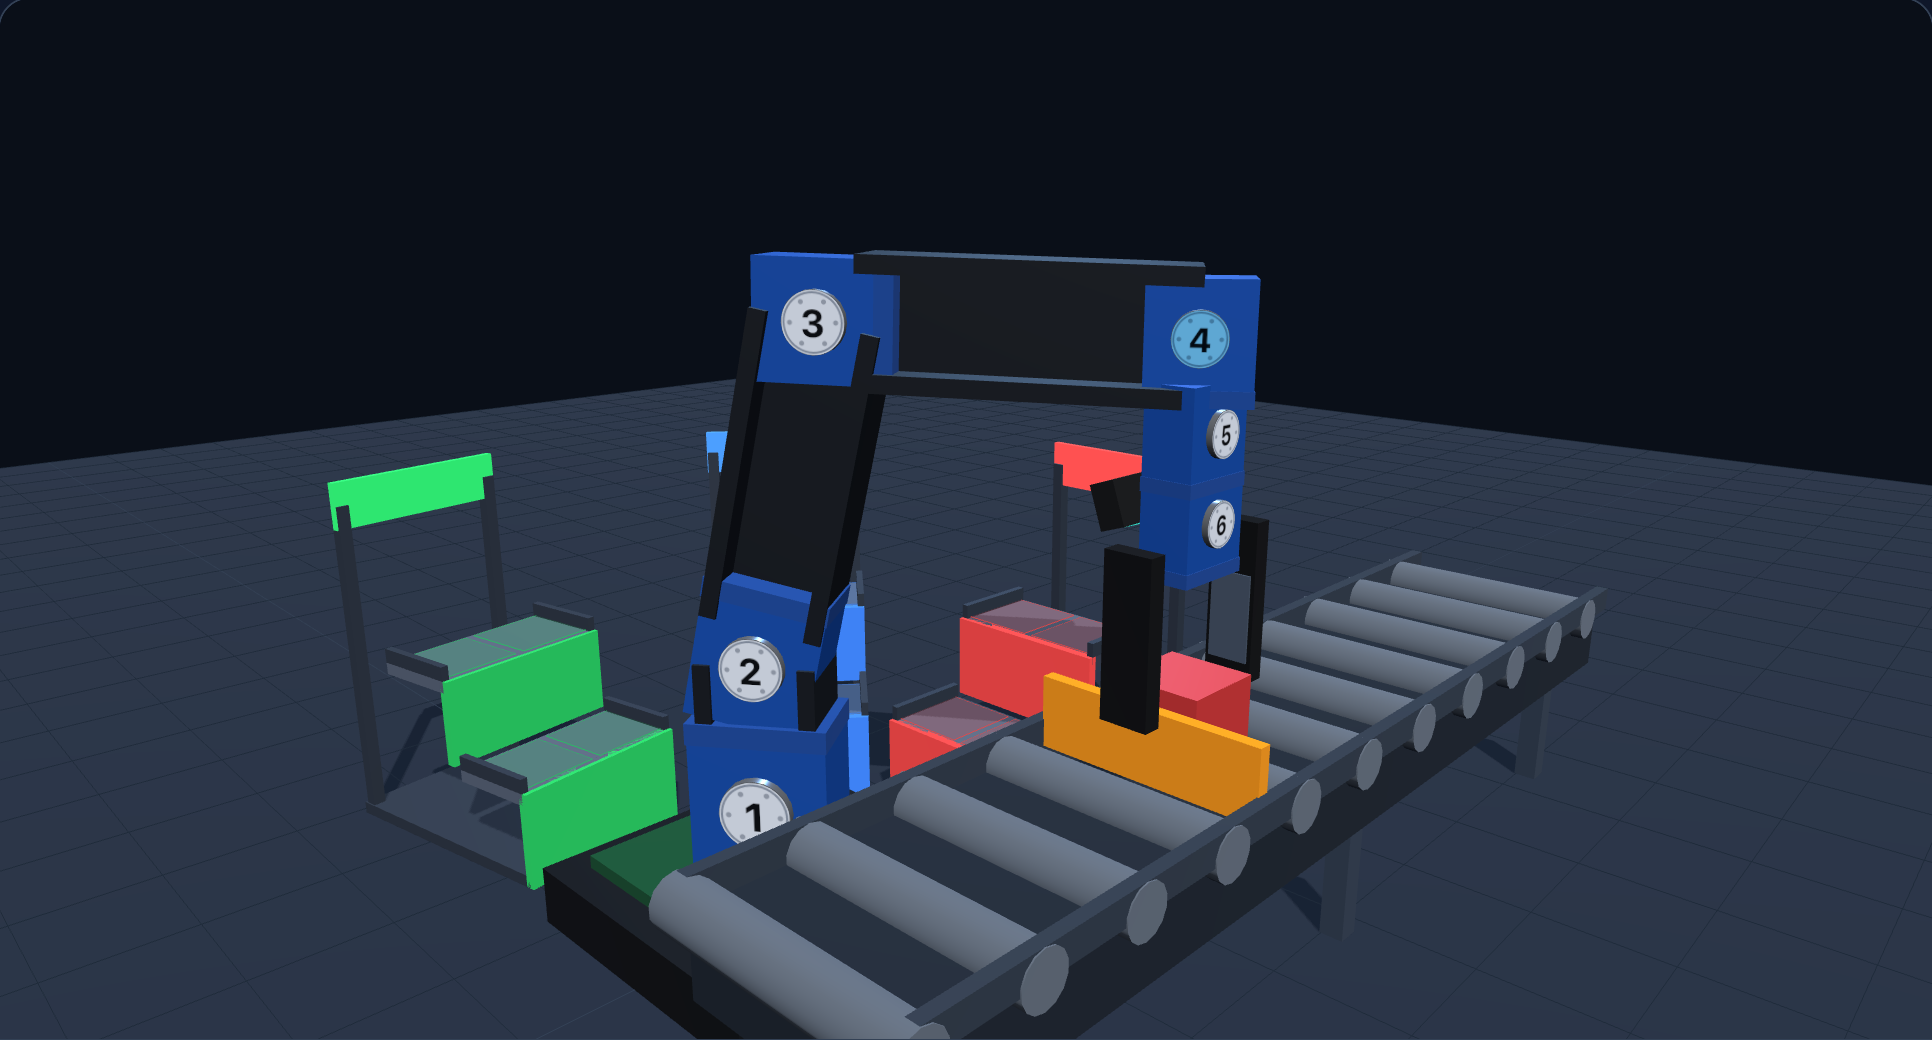
\includegraphics[width=0.86\textwidth]{fig/allsix.png}
\caption{作業セル。アーム中央、左が緑の棚、手前がコンベア。銀色ホーンの数字がサーボ ID
（ID4 が点灯＝駆動中）。棚は色ごとに 3 台、雛壇 2 段 $\times$ 2 スロット。}
\label{fig:servo}
\end{figure}

\section{Capability（効果）推論}

\subsection{仕組み}
AIPL の効果は \emph{gradual} である。処理系は各メソッド本体が呼ぶ一次作用（primitive）から
効果集合を観測し、ソースに申告がある場合に限り「申告 $\supseteq$ 観測」を検査する。
本作業で DOFBOT 実機デバイスのプリミティブを処理系へ追加し、次の効果を与えた。

\begin{center}
\small
\begin{tabular}{@{}l l l@{}}
\toprule
\textbf{プリミティブ} & \textbf{効果} & \textbf{根拠} \\
\midrule
\texttt{Arm\_serial\_servo\_write(id,angle,ms)} & \eff{mut} & 実機サーボを物理的に動かす \\
\texttt{Arm\_serial\_servo\_read(id)} & （なし） & 計測のみ。何も動かさない \\
\texttt{dofbot\_belt\_drive(cmd)} & \eff{mut} & コンベアもアクチュエータ \\
\texttt{dofbot\_camera\_grab()} & （なし） & センサ読取 \\
\texttt{tinyml\_load(path)} & \eff{fs} & 重みをファイルから読む \\
\texttt{tinyml\_infer(model,features)} & \eff{ai} & \textbf{net を持たない} \\
\bottomrule
\end{tabular}
\end{center}

\noindent
\texttt{tinyml\_infer} が \eff{ai} のみで \eff{net} を伴わない点は設計上の主張である。
既存の \texttt{ai\_call} 系（LLM 呼び出し）は \eff{ai, net} を持つ。両者を型で区別することで、
\emph{ローカル推論は機外へ何も出さない}ことをコードを読まずに保証できる。カメラ画像が
外部へ送信されないことが、\texttt{RecognitionActor} の効果集合から従う。

\subsection{効果推論が実際にバグを検出した}
本作業中、\texttt{ShelfActor.alloc} に \texttt{write\_file} を書きながら \eff{fs} を申告し忘れた。
処理系は即座にこれを指摘した。

\begin{lstlisting}[language=,basicstyle=\ttfamily\scriptsize]
$ ./aipl/run_aipl.sh check
[type] method ShelfActor.alloc: effect set incomplete
       -- declared {mut, net} but uses {fs}; missing: {fs}
\end{lstlisting}

\noindent
これは「効果注釈が飾りではない」ことの実証である。最終的に永続化を
\texttt{SafetyActor} へ集約し、現在は次のとおり指摘ゼロである。

\begin{lstlisting}[language=,basicstyle=\ttfamily\scriptsize]
$ ./aipl/run_aipl.sh check
[type] no issues.
\end{lstlisting}

\subsection{ブラウザ側の推論との一致}
シミュレータ画面のアクターカードは、\emph{申告を読まずに}メソッド本体の primitive から
効果を独立に推論して表示する。11 クラス中 9 クラスで推論と申告が完全一致した。
残る 2 つ（\texttt{PlannerActor}, \texttt{Coordinator}）は申告のほうが広いが、これは正常である。
両者は呼び出し先から伝播する \eff{ai} を申告しており、処理系は呼び出し連鎖を追うのに対し、
ブラウザ側は直接の primitive しか見ないためである。

\section{TinyML --- 手首カメラによる認識}

\subsection{構成}
手首カメラはグリッパ脇に載る実カメラであり、$96\times96$ のレンダターゲットへ描画される。
読み出した画素がそのまま TinyML の入力になり、\emph{画面右上に表示しているのは
推論に渡すのと同一の画素}である。

\begin{center}
\small
\begin{tabular}{@{}ll@{}}
\toprule
入力 & $96\times96$ RGBA $\to$ 中央 62\% を切出し $\to$ $8\times8$ 平均プーリング $\to$ 192 次元 \\
構造 & $192 \to 12\,(\tanh) \to 3\,(\mathrm{softmax})$、\textbf{2{,}355 パラメータ} \\
学習 & 交差エントロピー + モーメンタム付き SGD。numpy/PyTorch 非依存の純 Python \\
データ & 実レンダ画像 600 枚（3 クラス各 200 枚）。姿勢・撮像高さ・部品の向きを振る \\
\bottomrule
\end{tabular}
\end{center}

\noindent
フレームワークに依存しないことが要点である。行列積を素で書いた数十行であり、
実機の Raspberry Pi でも Xinu 上でもそのまま動く規模に収めてある。
学習・シミュレータ推論・AIPL 推論の 3 者が同一の前処理関数を通る。

\subsection{カメラ劣化モデル}
初期の実装ではテスト精度が \emph{epoch 0 で 100\%} に達した。理想的すぎる画像に対し、
分類器が平均色だけで解いてしまい、何の仕事もしていなかったためである。
そこで実機の安価な USB カメラ相当の劣化を導入した（図\ref{fig:wrist}）。

\begin{itemize}[leftmargin=1.4em,itemsep=1pt]
  \item 露出ゆらぎ：ゲイン $\sim U(0.55, 1.45)$
  \item ホワイトバランス偏り：チャンネルごとに $\sim U(0.85, 1.15)$
  \item センサノイズ：$\sigma = 12/255$ のガウス雑音
\end{itemize}

\begin{figure}[t]
\centering
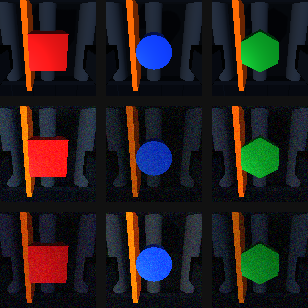
\includegraphics[width=0.52\textwidth]{fig/wrist_noise.png}
\caption{手首カメラの実画像（左から赤・青・緑）。上段は劣化なし、
中下段が実機相当の劣化モデル適用後。露出・色温度・ノイズがフレームごとに揺れる。
表示も推論もこの劣化後の画素を使う。}
\label{fig:wrist}
\end{figure}

\subsection{結果 --- 正直な評価}
劣化モデルを入れてもなお、\textbf{テスト精度は 100\%}（120 枚、混同行列は完全対角）であった。

\begin{center}
\small
\begin{tabular}{@{}lrrr@{}}
\toprule
正解 $\backslash$ 予測 & 赤 & 青 & 緑 \\
\midrule
赤・立方体 & \textbf{41} & 0 & 0 \\
青・円柱   & 0 & \textbf{37} & 0 \\
緑・六角柱 & 0 & 0 & \textbf{42} \\
\bottomrule
\end{tabular}
\end{center}

\noindent
\textbf{この結果は「難しい視覚課題を解いた」と読んではならない。} 3 色は彩度が高く、
色相は露出変動でも保たれるため、課題自体が本来易しい。モデルも学習も本物であり、
実レンダ画像から学習して実画素で推論しているが、色分けは元来容易なタスクである。
なお途中で 65.8\% という数値が出たが、これは課題の難しさではなく学習率 0.35 が
発散していた筆者のバグであり、0.02 で 100\% に戻った。

認識結果のみで棚が決まる点は重要である。部品の真の色は答え合わせにしか使っておらず、
\emph{誤認識すれば本当に違う色の棚へ運ばれる}。したがって後述の「色一致」検証は
視覚系の end-to-end 検証になっている。

\section{強化学習 --- サイクル時間の最小化}

\subsection{定式化}
方策 $\phi \in \mathbb{R}^{14}$ は幾何 3 次元と時間 11 次元からなる。
\[
\phi = (\underbrace{u_{\text{carry}},\; y_{\text{carry}},\; h_{\text{hover}}}_{\text{幾何}},\;
\underbrace{T_1, \ldots, T_{11}}_{\text{各フェーズの所要時間}})
\]
幾何を変えると全フェーズの関節変位が非線形に変わるため、時間だけを詰める問題ではない。
ここが Cross-Entropy Method (CEM) を用いる理由である。報酬は
\[
R(\phi) = -\,\overline{T_{\text{cycle}}}(\phi) \;-\; W \cdot \overline{V}(\phi), \qquad W = 50
\]
であり、$V$ は制約違反量である。制約は次のとおり。

\begin{itemize}[leftmargin=1.4em,itemsep=1pt]
  \item \textbf{サーボ角速度上限}：min-jerk 補間のピーク速度は平均の 1.875 倍であるから、
        各関節 $j$ について $1.875\,\Delta q_j / T \le v_{\max}$
  \item \textbf{可動域}：全サーボ指令角が $0\text{--}180^\circ$
  \item \textbf{到達性}：全ポーズが逆運動学で解ける
  \item \textbf{干渉}：旋回搬送中に棚および既設部品と当たらない
  \item \textbf{グリッパ最小開閉時間}：$0.18$ 秒
\end{itemize}

\noindent
評価は 12 スロット全部を巡る決定論的タスク集合であり、乱数で有利不利が出ない。
$W$ を十分大きく取り、\emph{違反が残る解は採用しない}（適用スクリプトが拒否する）。
これは重要で、罰則が小さいと最適化は「少し制約を破って時間を稼ぐ」解を選ぶ。
実際 $W$ が小さい設定では違反 0.141 を残した解が最良となった。

\subsection{結果}

\begin{figure}[t]
\centering
\begin{tikzpicture}
\begin{axis}[
  width=0.66\textwidth, height=5.4cm,
  xlabel={世代}, ylabel={サイクル時間 [秒]},
  xmin=0, xmax=119, ymin=4.8, ymax=8.0,
  axis y line*=left, axis x line*=bottom,
  grid=major, grid style={black!10},
  legend pos=north east, legend style={draw=none, fill=none, font=\small},
]
\addplot[thick, blue!70!black] table[x=gen, y=cycle] {rl_curve.dat};
\addlegendentry{学習中の方策}
\addplot[dashed, red!70!black, domain=0:119] {6.3};
\addlegendentry{手調整 6.300 秒（ただし実機で成立せず）}
\addplot[dotted, black!60, domain=0:119] {3.9044};
\addlegendentry{速度制限からの下界 3.904 秒}
\end{axis}
\end{tikzpicture}
\caption{CEM の収束。第 0 世代は制約違反 1.105 を含むため時間が長く見えるが、
第 10 世代以降は違反 0 を保ったまま短縮している。}
\label{fig:rl}
\end{figure}

\begin{center}
\small
\begin{tabular}{@{}lrr@{}}
\toprule
 & \textbf{手調整} & \textbf{学習後} \\
\midrule
サイクル時間 & 6.300 秒 & \textbf{5.164 秒}（$-18.0\%$） \\
制約違反 & \textbf{3.152} & \textbf{0.000} \\
搬送引込半径 $u_{\text{carry}}$ & 0.750 & 0.722 \\
搬送高さ $y_{\text{carry}}$ & 1.900 & 1.539 \\
ホバー高さ $h_{\text{hover}}$ & 0.400 & 0.239 \\
\bottomrule
\end{tabular}
\end{center}

\subsection{最も重要な発見 --- ベースラインは実機で動かなかった}

表中の「制約違反 3.152」は誤植ではない。\textbf{手調整のベースラインは、実機のサーボが
出せない速度を要求していた。} 内訳は次のとおりである。

\begin{center}
\small
\begin{tabular}{@{}llrr@{}}
\toprule
フェーズ & サーボ & 要求ピーク角速度 & 上限比 \\
\midrule
⑪ ホームへ戻る & ID1 / ID5 & $347.0^\circ/\mathrm{s}$ & \textbf{1.93 倍} \\
⑥ 棚へ旋回 & ID1 / ID5 & $290.6^\circ/\mathrm{s}$ & \textbf{1.61 倍} \\
\bottomrule
\end{tabular}
\end{center}

\noindent
⑥旋回は ID1 を $155^\circ$ もの範囲で $1.0$ 秒で振る指令であり、上限 $180^\circ/\mathrm{s}$ の
1.61 倍に相当する。CG 上は何事もなく動くため、\emph{画面を見ている限り絶対に気づかない}。

強化学習の解は、この 2 フェーズを\textbf{遅く}した（⑥旋回 $1.00 \to 1.63$ 秒、
⑪ホーム $0.70 \to 1.36$ 秒）うえで、余裕のあったフェーズを大きく詰めている
（③下降 $0.50 \to 0.13$ 秒、⑧設置 $0.50 \to 0.14$ 秒、⑩退避 $0.45 \to 0.14$ 秒）。
すなわち得られたのは単なる高速化ではなく、\textbf{実機で成立する動作でありながら、
成立しなかった従来より速い}動作である。

\subsection{学習した方策の実装への反映と実測}
学習結果は \texttt{rl/apply\_policy.py} により \texttt{src/layout.js}（3D シミュレータ）と
\texttt{aipl/dofbot\_xinu.abcl}（実機へ出る \texttt{ms} 指令）の\emph{両方}へ書き戻される。
書き戻した後、実際にシミュレータを走らせてサイクル時間を実測した。

\begin{center}
\small
\begin{tabular}{@{}lr@{}}
\toprule
実測サイクル時間（3D シミュレータ実走行） & 5.215 秒 \\
方策の設定値 & 5.164 秒 \\
差 & 0.051 秒 \\
\bottomrule
\end{tabular}
\end{center}

\noindent
短縮は学習側のモデル上だけの話ではなく、実際の描画・逆運動学・状態機械を通した
実走行でも再現されている。なお学習解は下界 $3.904$ 秒の 132\% であり、まだ余地はある。

\section{全体の効率と検証}

\subsection{1 サイクルの AIPL}
\texttt{PlannerActor.run\_one} が作業の全体である。駆動も永続化も持たないことに注意されたい。

\begin{lstlisting}[language=AIPL]
method run_one() !{ai, net} {
  var st = now belt.arrived();              // ストッパで部品が止まっている

  now claw.write(180, 195);                 // (1) グリッパを開く
  var qa = now kin.solve(STX, STY + HOVER, STZ);
  now mover.to(qa, 380);                    // (2) 部品の真上へ(撮像姿勢)

  var frame = now camera.capture();         // 手首カメラで撮像
  var res   = now recog.classify(frame);    // TinyML 認識 -> ai
  var cls   = res[0];
  var slot  = now shelf.alloc(cls);         // 色の一致する棚の空き枠
  var P     = now kin.slot_pose(cls, slot);

  var qg = now kin.solve(STX, STY, STZ);
  now mover.to(qg, 130);                    // (3) 把持点まで下降
  now claw.write(105, 195);                 // (4) 把持(部品幅ぶんだけ閉じる)
  ...
  now mover.to(cr, 1631);                   // (6) 棚の方向へベース旋回
  ...
  send safety.complete(cls, slot);          // 永続化は SafetyActor の仕事
  var fd = now belt.feed();                 // 次の部品を停止位置へ
  reply(cls);
}
\end{lstlisting}

\noindent
このソースは実際に処理系で実行され、実機と同じ API へサーボ指令を出す。

\begin{lstlisting}[language=,basicstyle=\ttfamily\scriptsize]
$ ./aipl/run_aipl.sh
[dofbot] 12 Xinu(6サーボ x 2) + TinyML 起動。
[servo] ID6 ->  180.0deg in  195ms
[servo] ID1 ->    8.0deg in  380ms
[servo] ID2 ->   97.4deg in  380ms
  TinyML 認識 -> 緑・六角柱 信頼度 99.9%
[belt ] feed
[dofbot] 6 サイクル完了。サーボ指令 258 回。
\end{lstlisting}

\subsection{検証}
主張はすべて機械検査に紐づけてある。

\begin{center}
\small
\begin{tabularx}{\textwidth}{@{}l >{\raggedright\arraybackslash}X l@{}}
\toprule
\textbf{検査} & \textbf{内容} & \textbf{結果} \\
\midrule
\texttt{cell.mjs} & 全 12 スロット + コンベアの到達性、棚どうし・棚とコンベア・搬送経路・
グリッパと背板の干渉、サーボ可動域 & 干渉 0・到達不能 0 \\
\texttt{verify.mjs} & 実走行。把持点↔部品中心の距離、搬送中の追従、置いた棚の色一致、
設置誤差、全フェーズ実行 & 全項目合格 \\
\texttt{aipl\_sync.mjs} & ブラウザ側と AIPL の字面結合（クラス名・primitive・行対応・効果） & 同期 \\
\texttt{cycle\_time.mjs} & サイクル時間の実測と設定値の一致 & 差 0.051 秒 \\
\texttt{fault.mjs} & カメラ障害注入 $\to$ 不良品排出 $\to$ 復帰 & 巡回維持 \\
\texttt{run\_aipl.sh check} & AIPL の型・効果検査 & \texttt{no issues} \\
\bottomrule
\end{tabularx}
\end{center}

\noindent
主要な実測値は次のとおりである。

\begin{center}
\small
\begin{tabular}{@{}lr@{}}
\toprule
把持誤差（指を閉じた瞬間の 把持点 $\leftrightarrow$ 部品中心） & \textbf{0.000 mm} \\
搬送中の追従誤差（最大） & \textbf{0.000 mm} \\
設置誤差（解放時の 部品 $\leftrightarrow$ スロット中心） & \textbf{0.000 mm} \\
TinyML 認識（実走行） & 6/6 正解 \\
色一致（置いた棚） & 全数一致 \\
サーボ指令角 & ID1--ID6 すべて $0\text{--}180^\circ$ 内 \\
\bottomrule
\end{tabular}
\end{center}

\noindent
把持誤差が厳密に 0 なのは、逆運動学が解析解であり、把持点が部品中心に一致した瞬間に
剛体固定（\texttt{attach}）しているためである。旧実装は関節角がハードコードされており、
把持点は $y \approx 4.9$ の空中にあった。部品（$y \approx 0.9$）には物理的に届いておらず、
部品をハンドへ補間で吸着させて「掴んでいるように見せて」いた。

\section{実機接続の経路}
\label{sec:real}

デバイス層はバックエンド差替え式であり、AIPL ソースは 1 行も変えずに実機へ向けられる。

\begin{center}
\small
\begin{tabular}{@{}ll@{}}
\toprule
\texttt{DOFBOT\_BACKEND=log} & （既定）指令を標準出力へ。実機非接続でも完走する \\
\texttt{DOFBOT\_BACKEND=armlib} & DOFBOT の Raspberry Pi 上で Yahboom \texttt{Arm\_Lib} を叩く \\
\texttt{DOFBOT\_BACKEND=http} & \texttt{DOFBOT\_URL} のブリッジへ POST（LAN 越し） \\
\bottomrule
\end{tabular}
\end{center}

\section{限界と前提}

本報告の主張を読む上で、次の 4 点を明示しておく。

\begin{enumerate}[leftmargin=1.6em,itemsep=2pt]
  \item \textbf{実機は動かしていない。} 物理の DOFBOT はネットワーク上に存在しない。
        \texttt{armlib} / \texttt{http} 経路は用意してあるが未検証である。
  \item \textbf{$v_{\max} = 180^\circ/\mathrm{s}$ は仮定であり、データシート値ではない。}
        Yahboom の 15kg バスサーボは無負荷で約 $300^\circ/\mathrm{s}$ とされるが、
        負荷とアーム慣性を見込んで derate した。\S5.3 の「ベースラインは実機で動かない」
        という結論はこの仮定に依存する。仮定を $300^\circ/\mathrm{s}$ に緩めれば
        ⑥旋回は成立し、⑪ホームのみが違反となる。
  \item \textbf{視覚課題は易しい。} テスト精度 100\% は課題の平易さの反映であり、
        TinyML の能力の証明ではない。
  \item \textbf{強化学習は解析的下界に届いていない。} 学習解は下界の 132\% である。
        また力学モデルは min-jerk のピーク速度による近似であり、トルク・慣性・
        バックラッシュを含まない。
\end{enumerate}

\section{再現手順}

\begin{lstlisting}[language=bash,basicstyle=\ttfamily\scriptsize]
# 3D シミュレータ
./run.sh                          # localhost:8022

# AIPL（本物の処理系で実行）
./aipl/run_aipl.sh check          # 型 + 効果検査
./aipl/run_aipl.sh                # 実行（サーボ指令を出力）

# TinyML
node rl/capture_dataset.mjs       # 手首カメラの実画像から学習データ
python3 rl/train_tinyml.py        # 学習 -> aipl/tinyml_model.json

# 強化学習
python3 rl/dofbot_rl.py           # CEM -> rl/rl_policy.json
python3 rl/apply_policy.py        # 方策を layout.js と .abcl へ書き戻す
python3 rl/apply_policy.py --restore   # 手調整へ戻す

# 検証（方策を書き戻したら必ず通す）
node test/cell.mjs                # 幾何: 到達性・干渉
node test/verify.mjs              # 実走行: 把持誤差・色一致
node test/aipl_sync.mjs           # ブラウザ側と AIPL のずれ
node test/cycle_time.mjs          # サイクル時間の実測
\end{lstlisting}

\section{結び}

本作業で得られたもののうち、価値の順に 3 点を挙げる。

第一に、\textbf{効果推論は実際に働いた}。\texttt{ShelfActor.alloc} の申告漏れは
人間のレビューではなく処理系が見つけた。効果を型に載せる主張は、
それが実装バグを捕まえたという一点で裏付けられる。

第二に、\textbf{強化学習は「速くする」以上のことをした}。副産物として、
手調整の動作が実機のサーボ速度を超えていたことを暴いた。これは CG を眺めていても、
コードを読んでも見つからない種類の誤りである。制約を明示的に書き下し、
それを破る解を採用しないと決めたことで初めて表に出た。

第三に、\textbf{TinyML は本物になったが、課題は易しかった}。手首カメラは実際に描画され、
分類器は実画素から学習され、その出力だけで棚が決まる。しかし精度 100\% は
課題の平易さを反映したものであり、そう読まれるべきである。

共通するのは、\emph{見た目では分からないものを機械に検査させると、
実装は必ず嘘をついている}ということである。棚は重なり、サーボは可動域に張り付き、
グリッパは背板を突き抜け、カメラは自分の筐体の内側を写し、
効果推論のパネルは例外も出さずに死んでいた。いずれも画面上は正常に見えていた。

\end{document}
